\documentclass{article}
\usepackage[margin=1.5cm,bottom=2cm]{geometry}
\usepackage{fancyhdr}
\usepackage{graphicx}
\pagestyle{fancy}

\begin{document}
\fancyhead[L]{ 
\includegraphics[width=2cm]{au_logo.png} }
\fancyhead[R]{PHYS 2240: General Physics I}
\fancyfoot[C]{\thepage}
\vspace*{0cm}
\begin{center}
	{\LARGE \textbf{Quiz 2}}
	%\vspace{0.25cm}
	%{\Large Due: Friday, September 11}
\end{center}

A 1400 kg car is driving at 20 m/s when the driver notices a stop sign 40 meters away. The driver hits the brakes, which apply a constant force of 8000 N. 
\begin{enumerate}

\item On the diagram below: draw arrows on the car indicating the direction of its instantaneous velocity and acceleration at some point after it started braking but before it has come to rest.\\ 
\begin{center}
	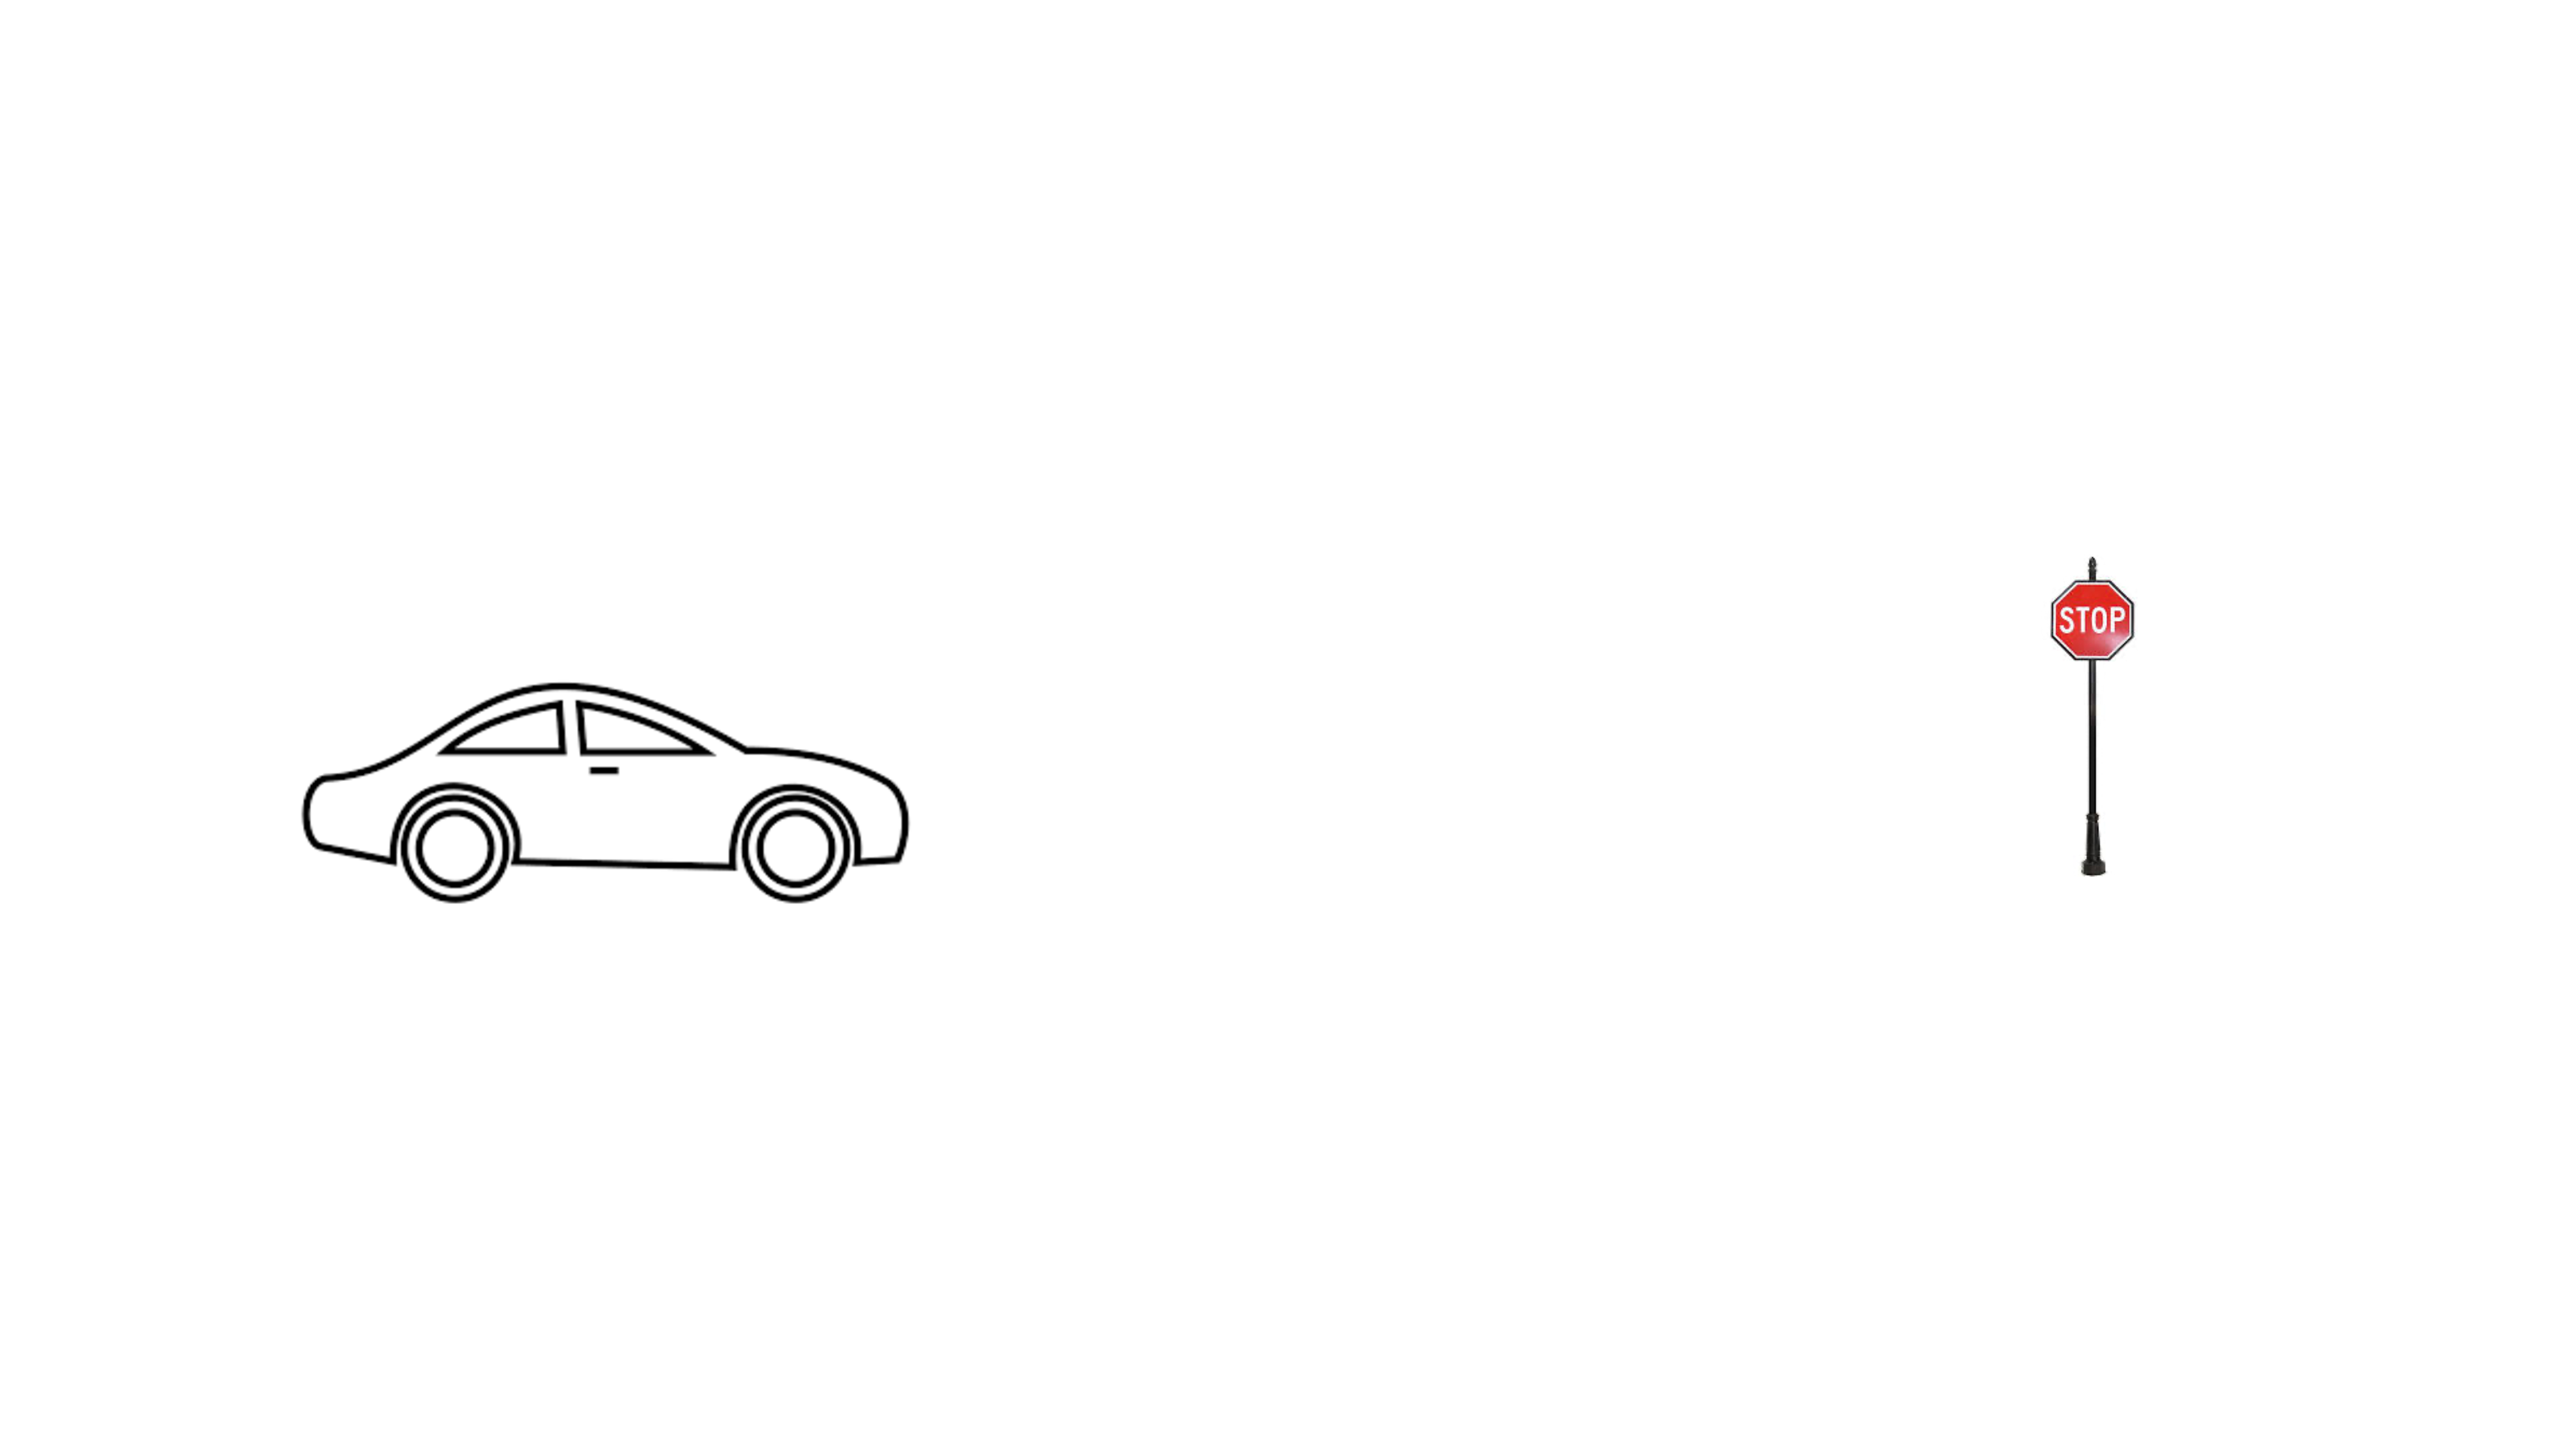
\includegraphics[width=10cm]{stupid.pdf}
\end{center}
\item Is the car able to stop before reaching the stop sign?\\
\textit{Show your work, do not just answer ``yes'' or ``no''. You should calculate the exact distance the car travels before coming to rest.}
\end{enumerate}

\end{document}